\subsection{Quản lý nhà thuê}
\subsubsection{Sơ đồ use-case}
\begin{figure}[H]
    \centering
    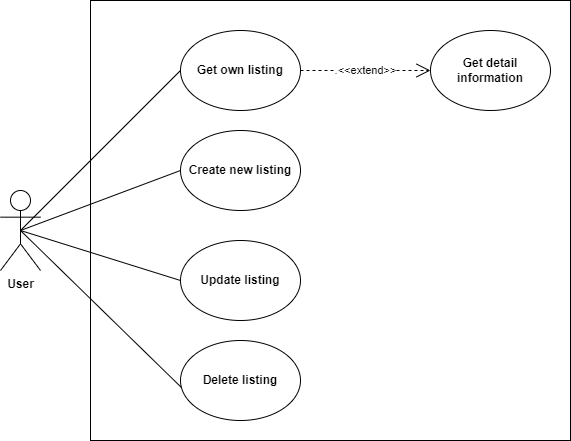
\includegraphics[width=0.7\textwidth]{Images/UseCase/ManageListing.png}
    \caption{Sơ đồ use-case cho chức năng quản lý nhà thuê}
\end{figure}
\subsubsection{Đặc tả use-case cho chức năng xem danh sách bài đăng tải nhà thuê của mình}
\begin{center}
    \arrayrulecolor{cyan!75!black}
    \arrayrulewidth=2pt
    \begin{longtable}{
        |>{\raggedright\arraybackslash}p{3cm}
        |>{\raggedright\arraybackslash}p{13cm}
        |}
        \hline
        \rowcolor{cyan!75!black} \textcolor{white}{\textbf{Use-case name}} & \textcolor{white}{\textbf{XEM DANH SÁCH BÀI ĐĂNG TẢI NHÀ THUÊ CỦA MÌNH}}
        \\\hline
        \rowcolor{cyan!10!white} \textit{Actor} & Người dùng
        \\\hdashline
        \rowcolor{cyan!10!white} \textit{Description} & Tính năng cho phép người dùng xem được danh sách các nhà thuê do mình đăng tải.
        \\\hdashline
        \rowcolor{cyan!10!white} \textit{Preconditions} & Người dùng đã đăng nhập thành công vào ứng dụng.
        \\\hdashline
        \rowcolor{cyan!10!white} \textit{Postconditions} & Kết quả được trả về thành công dưới dạng danh sách các bài đăng nhà thuê.
        \\\hdashline
        \rowcolor{cyan!10!white} \textit{Trigger} & Người dùng nhấn vào mục \textbf{Quản lý nhà thuê} ở trên giao diện ứng dụng
        \\\hdashline
        \rowcolor{cyan!10!white} \textit{Main flow} &
        1. Người dùng chọn vào mục \textbf{Quản lý nhà thuê}. \newline
        2. Ứng dụng truy vấn danh sách các nhà thuê do người dùng đăng tải. \newline
        3. Kết quả danh sách các bài đăng tải nhà thuê của người dùng được hiển thị thành công trên giao diện.
        \\\hdashline
        \rowcolor{cyan!10!white} \textit{Alternative flow} & Không có
        \\\hdashline
        \rowcolor{cyan!10!white} \textit{Exception flow} &
        \textbf{Nếu ứng dụng gặp lỗi khi thực hiện lấy ra danh sách bài đăng tải nhà thuê, ứng dụng thông báo lỗi và yêu cầu người dùng thử lại sau} \newline
        1a.1. Ứng dụng hiện lỗi khi thực hiện lấy ra danh sách bài đăng tải nhà thuê. \newline
        1a.2. Ứng dụng thông báo yêu cầu người dùng thử lại sau.
        \\\hline
        \caption{Đặc tả use-case cho chức năng xem danh sách bài đăng tải nhà thuê của mình}
    \end{longtable}
\end{center}
\subsubsection{Đặc tả use-case cho chức năng xem thông tin chi tiết về bài đăng tải nhà thuê của mình}
\begin{center}
    \arrayrulecolor{cyan!75!black}
    \arrayrulewidth=2pt
    \begin{longtable}{
        |>{\raggedright\arraybackslash}p{3cm}
        |>{\raggedright\arraybackslash}p{13cm}
        |}
        \hline
        \rowcolor{cyan!75!black} \textcolor{white}{\textbf{Use-case name}} & \textcolor{white}{\textbf{XEM THÔNG TIN CHI TIẾT VỀ BÀI ĐĂNG NHÀ THUÊ CỦA MÌNH}}
        \\\hline
        \rowcolor{cyan!10!white} \textit{Actor} & Người dùng
        \\\hdashline
        \rowcolor{cyan!10!white} \textit{Description} & Tính năng cho phép người dùng xem thông tin chi tiết về bài đăng tải nhà thuê của mình.
        \\\hdashline
        \rowcolor{cyan!10!white} \textit{Preconditions} & Người dùng đăng nhập thành công vào ứng dụng.
        \\\hdashline
        \rowcolor{cyan!10!white} \textit{Postconditions} & Thông tin chi tiết về một bài đăng tải nhà thuê của người dùng được hiển thị thành công trên ứng dụng.
        \\\hdashline
        \rowcolor{cyan!10!white} \textit{Trigger} & Người dùng chọn vào một bài đăng tải nhà thuê đang được hiển thị trên danh sách các bài đăng tải.
        \\\hdashline
        \rowcolor{cyan!10!white} \textit{Main flow} &
        1. Ứng dụng lấy ra các thông tin liên quan đến bài đăng tải nhà thuê. \newline
        2. Ứng dụng hiển thị thông tin chi tiết về bài đăng tải nhà thuê.
        \\\hdashline
        \rowcolor{cyan!10!white} \textit{Alternative flow} & Không có
        \\\hdashline
        \rowcolor{cyan!10!white} \textit{Exception flow} &
        \textbf{Nếu ứng dụng gặp lỗi khi hiển thị thông tin chi tiết của bài đăng tải nhà thuê, ứng dụng thông báo lỗi và yêu cầu người dùng thử lại sau} \newline
        1a.1. Ứng dụng hiện lỗi khi hiển thị lấy ra danh sách bài đăng tải nhà thuê. \newline
        1a.2. Ứng dụng thông báo yêu cầu người dùng thử lại sau.
        \\\hline
        \caption{Đặc tả use-case cho chức năng xem thông tin chi tiết về bài đăng tải nhà thuê của mình}
    \end{longtable}
\end{center}
\subsubsection{Đặc tả use-case cho chức năng tạo bài đăng tải nhà thuê}
\begin{center}
    \arrayrulecolor{cyan!75!black}
    \arrayrulewidth=2pt
    \begin{longtable}{
        |>{\raggedright\arraybackslash}p{3cm}
        |>{\raggedright\arraybackslash}p{13cm}
        |}
        \hline
        \rowcolor{cyan!75!black} \textcolor{white}{\textbf{Use-case name}} & \textcolor{white}{\textbf{TẠO BÀI ĐĂNG TẢI NHÀ THUÊ}}
        \\\hline
        \rowcolor{cyan!10!white} \textit{Actor} & Người dùng
        \\\hdashline
        \rowcolor{cyan!10!white} \textit{Description} & Tính năng cho phép người dùng tạo mới một bài đăng tải cho thuê nhà.
        \\\hdashline
        \rowcolor{cyan!10!white} \textit{Preconditions} & Người dùng đã đăng nhập thành công vào ứng dụng.
        \\\hdashline
        \rowcolor{cyan!10!white} \textit{Postconditions} & Thông tin về nhà thuê do người dùng nhập vào được đăng tải thành công.
        \\\hdashline
        \rowcolor{cyan!10!white} \textit{Trigger} & Người dùng chọn vào mục \textbf{Đăng tải nhà thuê} ở trên giao diện ứng dụng.
        \\\hdashline
        \rowcolor{cyan!10!white} \textit{Main flow} &
        1. Ứng dụng hiển thị các trường thông tin yêu cầu người dùng cung cấp khi đăng tải nhà thuê. \newline
        2. Người dùng nhập vào các trường thông tin đăng tải nhà thuê, có những trường thông tin bắt buộc được cung cấp và cũng có những trường thông tin có thể cung cấp hoặc không \newline
        3. Người dùng nhấn vào mục \textbf{Đăng tải nhà thuê}. \newline
        4. Ứng dụng kiểm tra và xử lý các trường thông tin do người dùng cung cấp. \newline
        5. Ứng dụng thông báo đăng tải nhà thuê thành công.
        \\\hdashline
        \rowcolor{cyan!10!white} \textit{Alternative flow} & 
        \textbf{Nếu người dùng hủy đăng tải nhà thuê, ứng dụng sẽ quay trở lại giao diện chính} \newline
        2a.1. Người dùng hủy quá trình đăng tải nhà thuê. \newline
        2a.2. Ứng dụng quay trở lại giao diện chính.
        \\\hdashline
        \rowcolor{cyan!10!white} \textit{Exception flow} & 
        \textbf{Nếu thông tin đăng tải nhà thuê không được cung cấp đầy đủ đối với các trường thông tin bắt buộc, ứng dụng sẽ hiển thị lỗi và yêu cầu người dùng cung cấp lại thông tin} \newline
        4a.1. Ứng dụng thông báo thông tin đăng tải nhà thuê chưa đầy đủ. \newline
        4a.2. Người dùng bổ sung thông tin đăng tải nhà thuê. \newline
        4a.3. Ứng dụng kiểm tra thông tin đã nhập. \newline
        4a.4. Nếu thông tin hợp lệ, ứng dụng sẽ thông báo đăng tải nhà thuê thành công, ngược lại sẽ quay lại bước 2. \newline
        \textbf{Nếu thông tin đăng tải nhà thuê không hợp lệ, ứng dụng sẽ hiển thị lỗi và yêu cầu người dùng cung cấp lại thông tin} \newline
        4a.1. Ứng dụng thông báo thông tin đăng tải nhà thuê không hợp lệ. \newline
        4a.2. Người dùng chỉnh sửa thông tin đăng tải nhà thuê. \newline
        4a.3. Ứng dụng kiểm tra thông tin đã nhập. \newline
        4a.4. Nếu thông tin hợp lệ, ứng dụng sẽ thông báo đăng tải nhà thuê thành công, ngược lại sẽ quay lại bước 2. \newline
        \textbf{Nếu ứng dụng gặp lỗi trong quá trình đăng tải nhà thuê, ứng dụng thông báo lỗi và yêu cầu người dùng thử lại sau} \newline
        4c.1. Ứng dụng hiện lỗi khi thực hiện đăng tải nhà thuê. \newline
        4c.2. Ứng dụng thông báo yêu cầu người dùng thử lại sau.
        \\\hline
        \caption{Đặc tả use-case cho chức năng tạo bài đăng tải nhà thuê}
    \end{longtable}
\end{center}
\subsubsection{Đặc tả use-case cho chức năng chỉnh sửa bài đăng tải nhà thuê}
\begin{center}
    \arrayrulecolor{cyan!75!black}
    \arrayrulewidth=2pt
    \begin{longtable}{
        |>{\raggedright\arraybackslash}p{3cm}
        |>{\raggedright\arraybackslash}p{13cm}
        |}
        \hline
        \rowcolor{cyan!75!black} \textcolor{white}{\textbf{Use-case name}} & \textcolor{white}{\textbf{CHỈNH SỬA BÀI ĐĂNG TẢI NHÀ THUÊ}}
        \\\hline
        \rowcolor{cyan!10!white} \textit{Actor} & Người dùng
        \\\hdashline
        \rowcolor{cyan!10!white} \textit{Description} & Tính năng cho phép người dùng chỉnh sửa thông tin của một bài đăng tải cho thuê nhà.
        \\\hdashline
        \rowcolor{cyan!10!white} \textit{Preconditions} & Người dùng đã đăng nhập thành công vào ứng dụng. Người dùng đã có ít nhất một bài đăng tải nhà thuê trên ứng dụng.
        \\\hdashline
        \rowcolor{cyan!10!white} \textit{Postconditions} & Thông tin về nhà thuê do người dùng nhập vào được cập nhật thành công.
        \\\hdashline
        \rowcolor{cyan!10!white} \textit{Trigger} & Người dùng chọn vào một bài đăng tải cho thuê nhất định và nhấn vào mục \textbf{Chỉnh sửa}.
        \\\hdashline
        \rowcolor{cyan!10!white} \textit{Main flow} &
        1. Ứng dụng hiển thị các trường thông tin hiện tại của bài đăng tải nhà thuê. \newline
        2. Người dùng nhập vào các trường thông tin muốn thay đổi đối với bài đăng tải nhà thuê. \newline
        3. Người dùng nhấn vào mục \textbf{Cập nhật thông tin}. \newline
        4. Ứng dụng kiểm tra và xử lý các trường thông tin do người dùng cung cấp. \newline
        5. Ứng dụng thông báo cập nhật thông tin nhà thuê thành công.
        \\\hdashline
        \rowcolor{cyan!10!white} \textit{Alternative flow} & 
        \textbf{Nếu người dùng hủy cập nhật thông tin nhà thuê, ứng dụng sẽ quay trở lại giao diện chính} \newline
        2a.1. Người dùng hủy quá trình cập nhật thông tin nhà thuê. \newline
        2a.2. Ứng dụng quay trở lại giao diện chính.
        \\\hdashline
        \rowcolor{cyan!10!white} \textit{Exception flow} & 
        \textbf{Nếu thông tin nhà thuê bị bỏ trống đối với các trường thông tin bắt buộc, ứng dụng sẽ hiển thị lỗi và yêu cầu người dùng cung cấp lại thông tin} \newline
        4a.1. Ứng dụng thông báo thông tin nhà thuê chưa đầy đủ. \newline
        4a.2. Người dùng bổ sung thông tin cho nhà thuê. \newline
        4a.3. Ứng dụng kiểm tra thông tin đã nhập. \newline
        4a.4. Nếu thông tin hợp lệ, ứng dụng sẽ thông báo cập nhật thông tin nhà thuê thành công, ngược lại sẽ quay lại bước 2. \newline
        \textbf{Nếu thông tin được ngươi dùng cập nhật không hợp lệ, ứng dụng sẽ hiển thị lỗi và yêu cầu người dùng cung cấp lại thông tin} \newline
        4a.1. Ứng dụng thông báo thông tin cập nhật không hợp lệ. \newline
        4a.2. Người dùng chỉnh sửa thông tin cập nhật nhà thuê. \newline
        4a.3. Ứng dụng kiểm tra thông tin đã nhập. \newline
        4a.4. Nếu thông tin hợp lệ, ứng dụng sẽ thông báo cập nhật thông tin thành công, ngược lại sẽ quay lại bước 2. \newline
        \textbf{Nếu ứng dụng gặp lỗi trong quá trình cập nhật thông tin nhà thuê, ứng dụng thông báo lỗi và yêu cầu người dùng thử lại sau} \newline
        4c.1. Ứng dụng hiện lỗi khi thực hiện cập nhật thông tin nhà thuê. \newline
        4c.2. Ứng dụng thông báo yêu cầu người dùng thử lại sau.
        \\\hline
        \caption{Đặc tả use-case cho chức năng chỉnh sửa bài đăng tải nhà thuê}
    \end{longtable}
\end{center}
\subsubsection{Đặc tả use-case cho chức năng xóa bài đăng cho thuê nhà}
\begin{center}
    \arrayrulecolor{cyan!75!black}
    \arrayrulewidth=2pt
    \begin{longtable}{
        |>{\raggedright\arraybackslash}p{3cm}
        |>{\raggedright\arraybackslash}p{13cm}
        |}
        \hline
        \rowcolor{cyan!75!black} \textcolor{white}{\textbf{Use-case name}} & \textcolor{white}{\textbf{XÓA BÀI ĐĂNG TẢI NHÀ THUÊ}}
        \\\hline
        \rowcolor{cyan!10!white} \textit{Actor} & Người dùng
        \\\hdashline
        \rowcolor{cyan!10!white} \textit{Description} & Tính năng cho phép người dùng xóa một bài đăng tải cho thuê nhà.
        \\\hdashline
        \rowcolor{cyan!10!white} \textit{Preconditions} & Người dùng đã đăng nhập thành công vào ứng dụng. Người dùng đã có ít nhất một bài đăng tải nhà thuê trên ứng dụng.
        \\\hdashline
        \rowcolor{cyan!10!white} \textit{Postconditions} & Bài đăng tải nhà thuê của người dùng được xóa thành công.
        \\\hdashline
        \rowcolor{cyan!10!white} \textit{Trigger} & Người dùng chọn vào một bài đăng tải cho thuê nhất định và nhấn vào mục \textbf{Xóa}.
        \\\hdashline
        \rowcolor{cyan!10!white} \textit{Main flow} &
        1. Ứng dụng hiển thị thông tin hiện tại của bài đăng tải nhà thuê. \newline
        3. Người dùng nhấn vào mục \textbf{Xóa bài đăng tải}. \newline
        4. Ứng dụng yêu cầu người dùng xác nhận việc xóa bài đăng tải. \newline
        5. Người dùng xác nhận việc xóa bài đăng tải. \newline
        6. Ứng dụng thông báo xóa bài đăng tải nhà thuê thành công.
        \\\hdashline
        \rowcolor{cyan!10!white} \textit{Alternative flow} & 
        \textbf{Nếu người dùng hủy xóa bài đăng tải nhà thuê, ứng dụng sẽ quay trở lại giao diện chính} \newline
        2a.1. Người dùng hủy quá trình xóa bài đăng tải nhà thuê. \newline
        2a.2. Ứng dụng quay trở lại giao diện chính.
        \\\hdashline
        \rowcolor{cyan!10!white} \textit{Exception flow} & 
        \textbf{Nếu ứng dụng gặp lỗi trong quá trình xóa bài đăng tải nhà thuê, ứng dụng thông báo lỗi và yêu cầu người dùng thử lại sau} \newline
        4c.1. Ứng dụng hiện lỗi khi thực hiện xóa bài đăng tải nhà thuê. \newline
        4c.2. Ứng dụng thông báo yêu cầu người dùng thử lại sau.
        \\\hline
        \caption{Đặc tả use-case cho chức năng xóa bài đăng tải nhà thuê}
    \end{longtable}
\end{center}